\begin{figure}[htbp]
\begin{center}
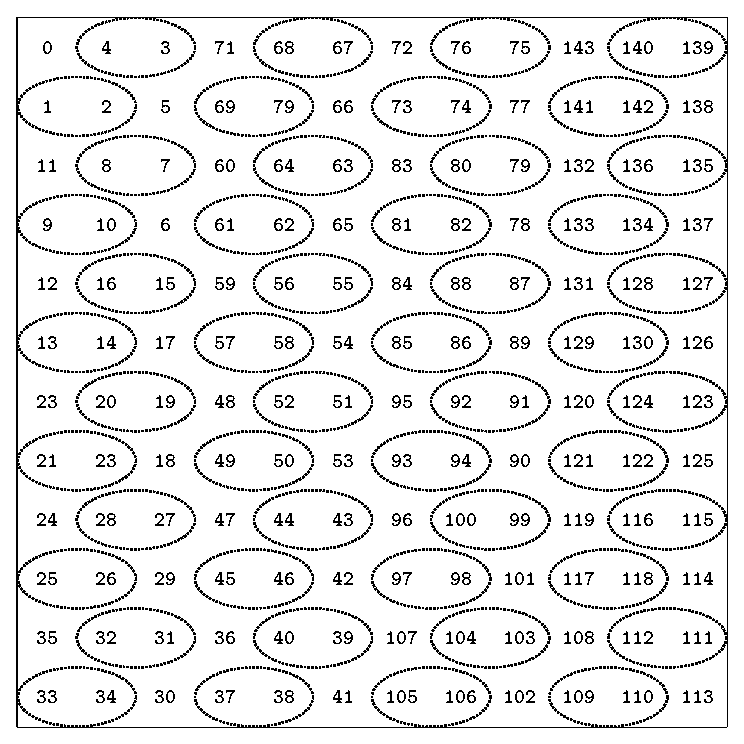
\includegraphics[scale=0.45]{order}
\caption{\small {\tt FFMA}s instruction scheduling to compute a $12\times 12$ sub-block of matrix C.  The numbers in
cells denote the {\tt FFMA} execution order. Dashed ellipses across two adjacent cells mean that two adjacent {\tt FFMA} instructions are dual issued in one clock cycle.}
\label{fig:order}
\end{center}
\end{figure}

\begin{figure}[htbp]
\begin{center}
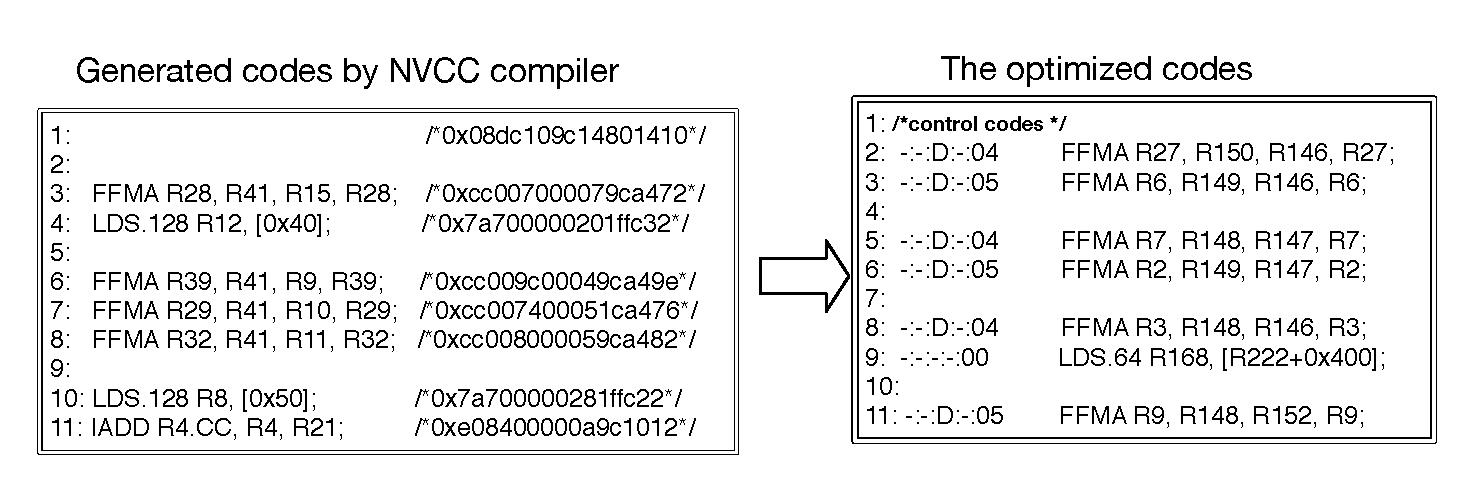
\includegraphics[scale=0.35]{assemlycode}
    \caption{\small The comparison of compiler generated codes and our tuned assembly codes.}
\label{fig:assemblycode}
\end{center}
\end{figure}
\subsection{FFMA Dual Issue}
\label{sec:ffma-dual}

It is unrealistic to keep warp schedulers dual issue the same kinds of arithmetic instructions (i.e., {\tt FFMA}) all
the time. Because on Kepler architecture, each warp is assigned $32$ cores privately, four warp schedulers will consume
$128$ cores. The reminding $192-128=64$ cores are divided into two 32-core groups, each $32$ cores
are shared by two warp schedulers. Two warp schedulers must negotiate who will use the extra $32$ shared cores to avoid
resource conflict.
As noted in {\em observation 3}, the best pattern of {\tt FFMA} instructions block is a sequence of one single issue(1
{\tt FFMA}), two dual issues (4 {\tt FFMA}s), and one single issue ((1 {\tt FFMA})). As shown in
Figure~\ref{fig:assemblycode}, the instructions in lines 3-4 and lines 6-7 are dual issued separately.
The other two instructions in line 8 and line 11 are two single issues in terms of floating-point instruction
execution.
As a comparison, most of the {\tt FFMA}s are single issued in the CUDA compiler generated codes.

By extending the basic $7$-instruction block (section~\ref{sec:benchmark}), we depict the scheduling pattern of computing a $12\times 12$ sub-block of matrix C in Figure~\ref{fig:order}.
% illustrates the order of $144$ {\tt FFMA}s instruction execution for calculating a $12\times 12$ subblock of matrix C.
For example, the {\tt FFMA} to calculate $C_{00}$ is issued first.
Then, two {\tt FFMA}s to
compute $C_{10}$ and $C_{11}$ are simultaneously issued. %We arrange all the {\tt FFMA} instructions of SGEMM according to the order in Figure~\ref{fig:order}.

Another advantage of this execution order is less register pressure due to register reuse, which can facilitate the
operand collector mechanism~\cite{collector}. The operand collector allows operand to be cached and reused in the subsequent instructions.
%is a storage element coupled with register file and
%provides inputs to the data path of the processor core for executing an instruction. %\jled{This is not the first occurrence of Operand collector.}
The assembly code in Figure~\ref{fig:assemblycode} lists the instructions to calculate $C_{32},C_{22}, C_{21}, C_{30},
C_{31}, C_{20}$, corresponding to the orders of $6,7,8,9,10,11$ in Figure~\ref{fig:reg}.
With the elaborately designed computing order and register allocation, the reuse happens as follows. The {\tt FFMA} in
Line $3$ uses cached operand {\tt R150} of line $2$, while Line $3$ and Line $4$ share {\tt R146}. Thus, in dual issue mode,
{\tt FFMA} of Line $3$ and $4$ need to read four registers {\tt R146}, {\tt R27}, {\tt R149}, {\tt R6} instead of six
registers. The corresponding banks of these registers are $0,1,3,2$ based on Table~\ref{tab:reg}, so no bank conflicts happen.
Similarly, Line 7 uses the cached operand {\tt R149} from the Line 4. In dual issue mode, two {\tt FFMAs} of Line 6 and
Line 7 need to read $4$ registers {\tt R148}, {\tt R147}, {\tt R7} and {\tt R2}.
